\documentclass[leqno,12pt]{book}

\usepackage{amsthm, amsfonts, amssymb, amsmath}
\usepackage{mystyle}
\usepackage{subfiles}
\usepackage{bookmark,rotating}

\usepackage[bibstyle=philosophy-modern,citestyle=philosophy-verbose,backend=biber,autopunct,sortcites,]{biblatex}
\DeclareNameAlias{sortname}{given-family}
\interfootnotelinepenalty=10000

\usepackage{iftex}

\ifxetex
	\usepackage{unicode-math}
	\newcommand{\fakebold}{1}
	\newcommand{\scale}{1}
	\newcommand{\fakemathbold}{1}
	\setmainfont[FakeBold=\fakebold,ItalicFont=ModernMT-ExtendedItalic-New.otf,ItalicFeatures={FakeBold=\fakebold,Scale=\scale},BoldItalicFont=ModernMT-ExtendedItalic-New.otf,SmallCapsFont={OldStandard-Regular.otf},SmallCapsFeatures={Letters=SmallCaps,FakeBold=\fakebold,RawFeature=+smcp,Scale=\scale},BoldFont=OldStandard-Bold.otf,BoldFeatures={FakeBold=0,Scale=\scale,SmallCapsFont=OldStandard-Bold.otf,SmallCapsFeatures={RawFeature=+smcp,Scale=\scale}},BoldItalicFeatures={FakeBold=3},]{ModernMT-Extended-New.otf}
	\setsansfont[FakeBold=1,Scale=\scale]{Latin Modern Sans}
	\setmonofont[FakeBold=1,Scale=\scale]{Latin Modern Mono}
	\setmathfont[FakeBold=\fakemathbold,Scale=\scale]{NewCMMath-Book.otf}
	\setmathfont[range={it,},FakeBold=\fakemathbold,Scale=\scale]{ModernMT-ExtendedItalic-New.otf}
	\setmathfont[range={up,},FakeBold=\fakemathbold,Scale=\scale]{ModernMT-Extended-New.otf}
	\setmathfont{texgyrepagella-math.otf}[range={"0028,"0029,"005B,"005D,"007B,"007D,}]
	%\setmathfont{OldStandard-Regular.otf}[range={"2A7D-"2A7E, "2AA1-"2AA2, "2AED,"3008-"300B,up},FakeBold=\fakemathbold]
	
	\newfontfamily{\bask}{ModernExtT-Theano.otf}
	\makeatletter
	\RenewDocumentCommand{\sum@}{}{\DOTSB\baskervillesum}
	\AtBeginDocument{%
		\RenewDocumentCommand{\sum}{}{\mathop{\sum@}\slimits@}%
	}
	\NewDocumentCommand{\baskervillesum}{}{%
		\mathchoice
		{\makebaskervillesum{1.8}}% displaystyle
		{\makebaskervillesum{1.2}}% textstyle
		{\makebaskervillesum{1}}% scriptstyle
		{\makebaskervillesum{0.7}}% scriptscriptstyle
	}
	\NewDocumentCommand{\makebaskervillesum}{m}{%
		\vcenter{\hbox{\scalebox{#1}{\bask Σ}}}%
	}
	\makeatletter
	\RenewDocumentCommand{\prod@}{}{\DOTSB\baskervilleprod}
	\AtBeginDocument{%
		\RenewDocumentCommand{\prod}{}{\mathop{\prod@}\slimits@}%
	}
	\NewDocumentCommand{\baskervilleprod}{}{%
		\mathchoice
		{\makebaskervilleprod{1.5}}% displaystyle
		{\makebaskervilleprod{1.2}}% textstyle
		{\makebaskervilleprod{1}}% scriptstyle
		{\makebaskervilleprod{0.7}}% scriptscriptstyle
	}
	\NewDocumentCommand{\makebaskervilleprod}{m}{%
		\vcenter{\hbox{\scalebox{#1}{\bask ∏}}}%
	}
	\newfontfamily\intfont{OldStandard-Italic.otf}
	\makeatletter
	\NewDocumentCommand{\int@}{}{\DOTSB\baskervilleint}
	\AtBeginDocument{%
		\RenewDocumentCommand{\int}{}{\mathop{\int@}\slimits@}%
	}
	\NewDocumentCommand{\baskervilleint}{}{%
		\mathchoice
		{\makebaskervilleint{1.5}}% displaystyle
		{\makebaskervilleint{1.2}}% textstyle
		{\makebaskervilleint{1}}% scriptstyle
		{\makebaskervilleint{0.7}}% scriptscriptstyle
	}
	\NewDocumentCommand{\makebaskervilleint}{m}{%
		\vcenter{\hbox{\scalebox{#1}{\intfont ∫}}}%
	}
	\defaultfontfeatures{Mapping=tex-text,Ligatures=Tex}
\else
	%\usepackage{pdfrender, xcolor}
	\renewcommand*\rmdefault{cmdh}
	\usepackage[T1]{fontenc}
\fi

\usepackage{tocloft}
\renewcommand{\cftsecfont}{\normalsize\normalfont}
\renewcommand{\cftchapfont}{\normalsize\normalfont}
\renewcommand{\cftsubsecfont}{\normalsize\normalfont}
\renewcommand{\cftpartfont}{\normalsize\normalfont}

\usepackage[toc,nopostdot,nonumberlist,automake=true]{glossaries}
\usepackage{makeidx}

\usepackage{nomencl}
\renewcommand{\nomname}{Notations}
\makenomenclature
\glstoctrue
\subfile{glossary.tex}
\makeindex
\makeglossaries

\titleformat{\chapter}[display]{\bfseries\scshape\Huge}{}{1ex}{\centering\titlerule\vspace{1ex}\ifthenelse{\value{chapter}>0}{$\S\S$\thechapter\;}{}}[\vspace{1ex}\titlerule]
\titleformat{\section}[display]{\bfseries\scshape\LARGE}{}{1ex}{\centering\ifthenelse{\value{section}>0}{$\S\S$\thesection\;}{}}[\titlerule]
\titleformat{\subsection}[display]{\bfseries\scshape\Large}{}{1ex}{\centering\ifthenelse{\value{section}>0}{$\S\S\S$\thesection\;}{}}[\titlerule]
\renewcommand*{\chapterautorefname}{Chapter}
\renewcommand*{\sectionautorefname}{Section}
\renewcommand*{\subsectionautorefname}{Subsection}

\newcommand*{\problemautorefname}{\textit{Problem}}
\newcommand{\identityautorefname}{Identity}
\newcommand{\lemmaautorefname}{\textit{Lemma}}
%\renewcommand{\theoremautorefname}{\textit{Theorem}}

\title{\bf\Huge TOPICS IN NUMBER THEORY\\ {\vspace*{.3in}\it\LARGE An Olympiad--Oriented Approach}\\\vspace*{.3in}{\Large Second Edition\\\vspace*{.1in}\rule{\textwidth}{0.8pt}}}
\author{
	\Huge Masum Billal
	\and \Huge Amir Parvardi
	\\\vspace*{.4in}
	\rule{\textwidth}{0.8pt}\\\vspace*{.2in}
}
\date{}

\addbibresource{ref.bib}

\begin{document}
\pagestyle{empty}
\begin{tikzpicture}[remember picture,overlay]
	\node at (current page.center) {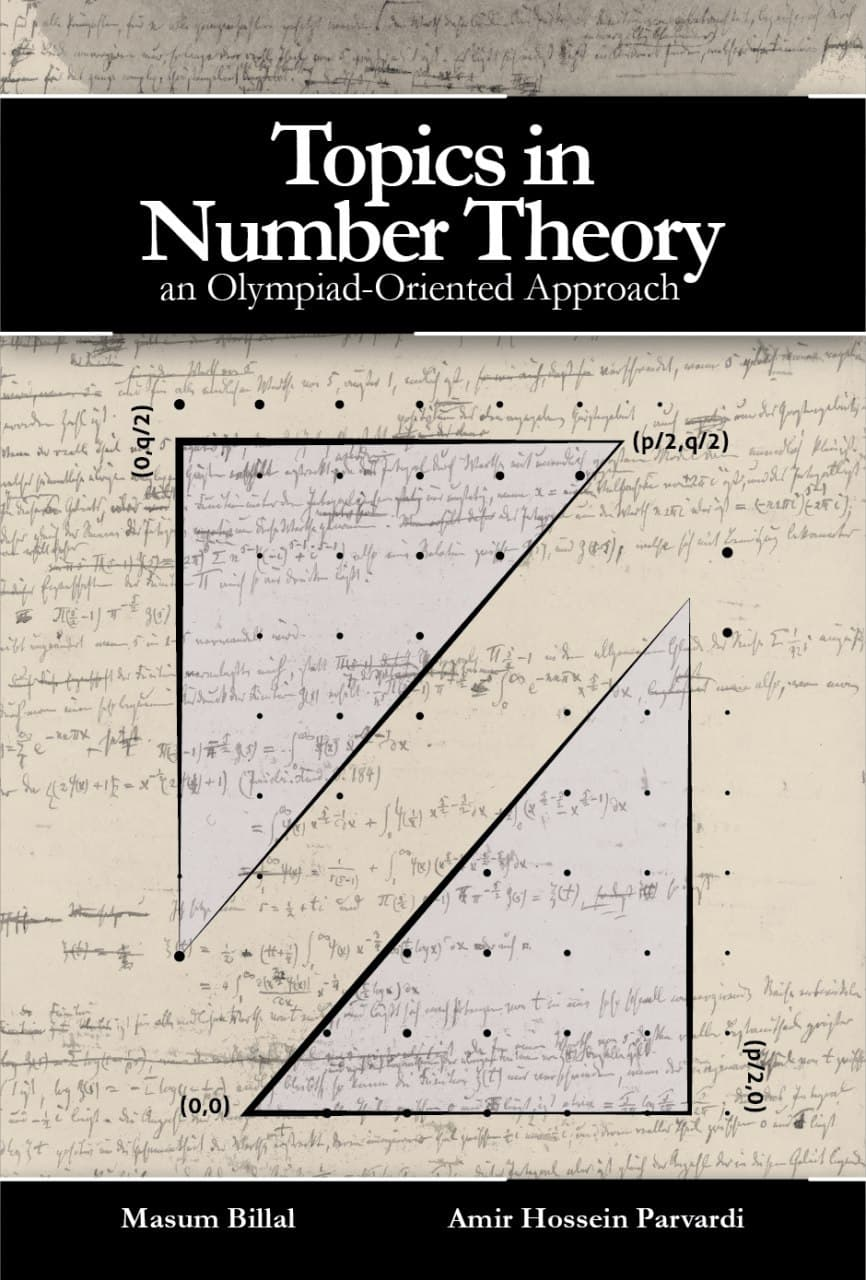
\includegraphics[origin=c,angle=0,width=\pdfpagewidth,height=\pdfpageheight]{TNT_Cover/FrontCover.jpg}};
\end{tikzpicture}
%\relsize{1.1}
\maketitle
\pagestyle{empty}
\frontmatter

\begin{dedication}
	\begin{center}
		\textit{Dedicated to}
	\end{center}
	Fermat, the father of modern number theory.\\
	Euler, without whom number theory probably wouldn't be so rich today.\\
	Ramanujan, the mathematician of mathematicians.\\
	Paul Erd\H{o}s, the man who loved only numbers.
\end{dedication}

\section*{Preface to Second Edition}
It has been over $3$ years since we have written this book. When we read the book now, we sometimes feel kind of silly. In some places, the writing comes off as childish and probably even unprofessional. But we do not regret writing the book that way. There are reasons why we have written it the way we did. We admit that we did not have the enormous amount of patience required to finish the book in a greater style. We were hurried to write a lot of the things back then. Not because we were told to, since this is an independent publication after all. There are a number of factors why we felt hurried to finish the book. For example, the book was already large even though we discarded a lot of the content we had planned for the book. In fact, we discarded most of the content we planned because the book would be so huge not even us would have been interested in reading a book that large. But that messed with our plans a lot since we had to change a lot of things on the fly. The whole reason we wanted to write a book despite there existing a lot of books on number theory is that we wanted our book to contain results or techniques that would not be as common in other Olympiad books. However, even with the minimum amount of content we decided to go with, it still felt like it was getting too large. So we tried to pick up the pace after some chapters. And one of the biggest concerns we had was that if we had not finished the book soon, we might not have been able to finish it at all. Or even worse, we could have forgotten about the whole book altogether (that has happened as well). Anyway, we mention these here not to make any excuses, nor do we feel terrible about it. Because even though the end-product does not look like the best output right now, we believe this book can still help people, at least some new students who are looking to solve number theory problems. Would the book be a lot better if we rewrote it now? Yes, probably at least ten times better. But we have neither the energy nor the time to do so. There are some updates and error fixes in this edition which hopefully improves at least some aspects of the book.

It is possible there are some \LaTeX\ issues in the new edition. If anyone finds any, please do not hesitate to email us.

\begin{flushright}
	\it Masum Billal\\
	Amir Parvardi\\
	August, $2021$
\end{flushright}
\section*{Links, Contact}


\newpage
\section*{Preface from first edition}

I would like to have a few words before diving into the discussion. First of all, from my personal experience, I have found that there is a common practice to learn by learning a lot of theories and then investigating how those theories are used to solve problems. As our primary audience would be students who are looking to get into mathematical Olympiads, I highly discourage this. Please do not take number theory for a collection of theories just because the word theory is literally juxtaposed with it. That being said, one could argue our book itself is a collection of a lot of theorems as well. Sadly, that is partially true for multiple reasons though it was not our intention at all.


When I first thought about writing this book, my intention was to make students realize that they do not need to know a lot of theorems in order to be able to solve problems. But as we kept writing, we had to increase the pace since we had to cover a lot (and that was discarding a lot of content which we thought would ask for even discussion or we just felt lazy about it), we had to increase the pace.


Initially, my plan was to make this book a series of $5$ volumes, this being the first one. In those volumes, I wanted to discuss a lot of topics such as special numbers like \textit{egyptian fraction} or even interesting numbers like \textit{abundant number or deficient number} and their properties, etc., or crucial topics such as \textit{Diophantine equations}. You will notice that we have left a lot of important topics like those out of this book. The reason is, I quickly realized I could hardly finish writing this first volume, and if I wanted to complete the whole series, we would probably have to keep writing my whole life. So, I had to discard a lot of content and make the book concise. This resulted in squeezing in a lot of content in a few hundred pages.


Finally, I would like to thank Amir for joining me in this project. At one point, I stopped writing the book. If he had not agreed to be a co-author, this book would have probably not been completed at all, more so because he agreed to follow the style I wanted to write in even when we had objections from a reputed publisher like \textit{Springer}.

\begin{flushright}
	\sl Masum Billal
\end{flushright}

\newpage

In the past three years, we have always been worried about this book. It's been a long and tedious job to manage everything and edit all we had written a very long time ago. After I studied more number theory concepts of higher level, there were times that I found errors/typos in my previous drafts for the book. And that sometimes happened two or more times in a short period, and so, it was getting annoying. Anyhow, we managed to finish it at this time of the summer. It is now 5:36 AM, Tuesday, July 17, 2018, that I'm writing this. You can imagine how crazy this process has made me!

\vspace{0.3cm}
Many of our friends helped us on the way to finish this book, as mentioned in the acknowledgment, and we are so proud to have such friends. I wouldn't be able to finish my part in this book if I didn't have the support of my wonderful, beautiful, and lovely wife \textit{Nadia Ghobadipasha}. She gave me hope to choose mathematics and always believed in me. She was the only one in the hardest days of my life.
\vspace{0.3cm}
Professor \textit{Peyman Nasehpour}, whom I knew from the very first semester of my undergraduate studies in electrical engineering at the University of Tehran, helped me a lot in the process of enhancing my mathematical abilities to change my field to mathematics (number theory) for my master's.  He is an inspiration and a great colleague to me when it comes to teamwork. I'm looking forward to working with him more often.
\vspace{0.3cm}
The idea behind the lattices in the \textit{cover} is a geometric proof of the law of quadratic reciprocity. Our friends found other interpretations such as the Pick's theorem (which is not the case here) or the sum of positive integers up to $n$, which you will realize is also not always true (for all primes $p,q$). Section \eqref{sec:qrlawproof} is dedicated to this proof and investigates why it is true using counting the lattice (grid) points. When we picked this idea for the cover, we chose quadratic reciprocity because its proof is geometrically visual and indeed very beautiful. Our hope was to make the reader curious because the design looks familiar. I remember I found the idea of the proof in one of Kenneth H. Rosen's books on discrete mathematics, but I'm not sure which one, as it was a long time ago when I wrote it. I used the TikZ package for \LaTeX to write the codes and generate the graphs.
\vspace{0.3cm}
There are so many wonderful things to learn in this book. I hope you enjoy it!
\begin{flushright}
	\sl Amir Parvardi,\\
% 	University of British Columbia,\\
	Vancouver, BC, Canada,\\
	July 2018.
\end{flushright}

\newpage

\section*{Acknowledgment}

Here is a list of all the kind people who helped us review, edit, and improve this book. The list is ordered alphabetically based on the last name.
	\begin{enumerate}
		\item Thanks to \textit{Ali Amiri}, a kind friend who helped us with the cover design.
		\item Thanks to \textit{Anr\'{e}C} from TeX.StackExchange who wrote the code for figure \eqref{fig:base16} in base conversion.
		\item We are thankful to \textit{Arta Khanalizadeh} for designing the cover of the book.
		\item Thanks to \textit{Kave Eskandari} for reading the whole book and commenting on the general points. He caught a good mistake in chapter \ref{ch:divisibility}.
		\item Cheers to our mathematical friend \textit{Leonard Mihai C. Giugiuc} from Romania that gave us positive and constructive feedback on the book. He also wrote us a wonderful review on the website.

		\item Thanks to \textit{Valentio Iverson} for proof-reading chapters \ref{ch:arithfunc} and \ref{ch:special}, and pointing out the typo in figure \eqref{fig:unitfunction}.

		\item Thanks to \textit{Aditya Khurmi} for reading the book and giving us positive feedback.

		\item We appreciate \textit{Hesam Korki}'s comments on chapter \ref{ch:divisibility}. He mentioned a few very important typos, including grammatical. He also mentioned a mathematical change of that chapter, which was very helpful.

		\item Professor \textit{Peyman Nasehpour} sent us the beautiful problem \eqref{prob:nasehpour} and an amazing solution using Prime Number Theorem. He also gave us pretty useful comments on chapter \ref{ch:divisibility}. He also introduced in section \eqref{sec:sum-of-divisors} the amicable numbers to us with a brief historical note on it.

		\item We appreciate \textit{Kenji Nakagawa}'s comments on chapters \ref{ch:primes} and \ref{ch:special}. He was one of the first people who read and reviewed these two chapters when we put them on the website of the book.

		\item We are thankful towards \textit{Mohammadamin Nejatbakhshesfahani}, Iran National Olympiad gold medalist (2010) and winner of gold medals at IMS and IMC, who honored us to read and review the whole book and gave us really instructive comments.

		\item We would like to thank \textit{Nur Muhammad Shafiullah Mahi} for his efforts to make this book better.

		\item We are honored to thank Professor \textit{Greg Martin}, a faculty member at the Mathematics Department of the University of British Columbia. He happens to be Amir Hossein's Master's supervisor. He kindly reviewed a printed draft of the book and emailed us over $10$ major points to correct in the book. We do appreciate his advice on improving the whole context of the book.

		\item We are thankful to \textit{Sohrab Mohtat} for his comments on chapter \ref{ch:divisibility}. Thanks to him, we avoided a fatal mistake at the beginning of the book. He also wrote a very useful and detailed review for our book on the website.

		\item We are thankful to \textit{Aditya Guha Roy} who reviewed the whole book and caught a few LaTeX typos, generalized lemma \eqref{lem:aditya-generalized}, fixing problems in chapter \ref{ch:unsolved}. Aditya wrote an amazing, educative review on our website.
		\item \textit{Navneel Singhal} carefully reviewed and proof-read the whole first part of the book (chapters \ref{ch:divisibility} to \ref{ch:special}) and gave us very constructive comments. We are thankful to him.

		\item Thanks to \textit{Amin Soofiani}, who is a Master's student of mathematics at the University of British Columbia, we noticed there was a mistake in theorem \eqref{thm:numofprime}. He did a perfect, precise, and detailed review on chapter \ref{ch:primes}.

		\item We are thankful to \textit{Sepehr Yadegarzadeh} for informing us about the correct \textit{umlaut}\footnote{\textit{umlaut}: a mark (\H{}), used over a vowel, as in German or Hungarian, to indicate a different vowel quality, usually fronting or rounding.} for M\"{o}bius among other grammatical and vocabulary points.
	\end{enumerate}
	\clearpage
	%\dominitoc
	\tableofcontents
	\subfile{nomenclature.tex}
	\printnomenclature
	\mainmatter
	\pagestyle{fancy}
	\setcounter{page}{13}
	%\begin{refsection}
		%\subfile{intro.tex}
		%\printbibliography
	%\end{refsection}
	%\minitoc \mtcskip \minilof
	%\begin{refsection}
		\subfile{divisibility.tex}
		%\printbibliography
	%\end{refsection}
	%\minitoc \mtcskip \minilof
	%\begin{refsection}
		\subfile{congruence.tex}
		%\printbibliography
	%\end{refsection}
	%\minitoc \mtcskip \minilof
	%\begin{refsection}
		\subfile{arithfunc.tex}
		%\printbibliography
	%\end{refsection}
	%\minitoc \mtcskip \minilof
	%\begin{refsection}
		\subfile{primes.tex}
		%\printbibliography
	%\end{refsection}
	%\minitoc \mtcskip \minilof
	%\begin{refsection}
		\subfile{special.tex}
		%\printbibliography
	%\end{refsection}
	%\resumechapters
	%\begin{refsection}
		\subfile{solved.tex}
		\subfile{unsolved.tex}
		\subfile{unsolved2016.tex}
		%\printbibliography
	%\end{refsection}

	\backmatter
	\pagestyle{empty}
	\printglossaries
	\printbibliography

\end{document}